%%%%%%%%%%%%%%%%%%%%%%%%%%%%%%%%%%%%%%%%%%%%%%%%%%%%%%%%%%%%%%%%%
\chapter{LORA \& LORAWAN}\label{ch:lora_lorawan}
%%%%%%%%%%%%%%%%%%%%%%%%%%%%%%%%%%%%%%%%%%%%%%%%%%%%%%%%%%%%%%%%%

\section{LoRa}

LoRa is a proprietary physical layer radio/chipset technology that provides wireless link solution for low power wide area networks. It uses proprietary spread spectrum modulation technique that is the derivative of Chirp Spread Spectrum (CSS). CSS was originally developed for radar applications in the 1940’s. A chirp is a sinusoidal signal of which frequency increases over time \cite{1091721}. Chirp frequency increases linearly and sweeps the entire bandwidth \cite{AN1200.22}.

\begin{figure}[h]
\centering
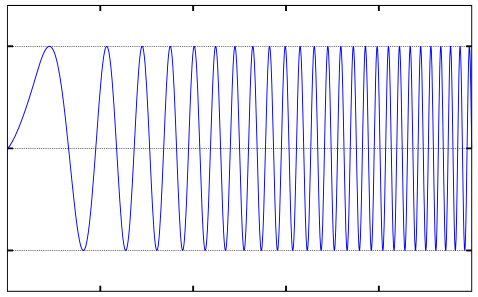
\includegraphics[width=.6\linewidth]{fig/lora_chirp.png}
\vspace*{5mm}
\caption{A CSS up-chirp in time domain. \cite{sghoslya_lora}}
\label{fig:lora_chirp}
\end{figure}

\subsection{Spreading Factor}

The ratio between symbol and chirp rate is equal to $2$\textsuperscript{SF}. Spreading factor can take values between 7 to 12. Spreading factor also determines data rate of a LoRa transmission \cite{AN1200.22}. Data rate of a LoRa transmission can be calculated as:

\begin{equation} \label{eq:bit_rate_sf}
R_{b} = SF * \dfrac{\left[ \dfrac{4}{4+CR} \right] }{ \left[ \dfrac{2^{SF}}{BW|_{Hz}} \right]} \ bps
\end{equation}

Where, $R_{b}$ is data rate in bps, SF is spreading factor $SF \in \{7,..,12\}$, CR is error correction code rate $CR \in \{1,..,4\}$ and $BW$ is bandwidth in Hertz \cite{AN1200.22}.

\begin{figure}
\centering
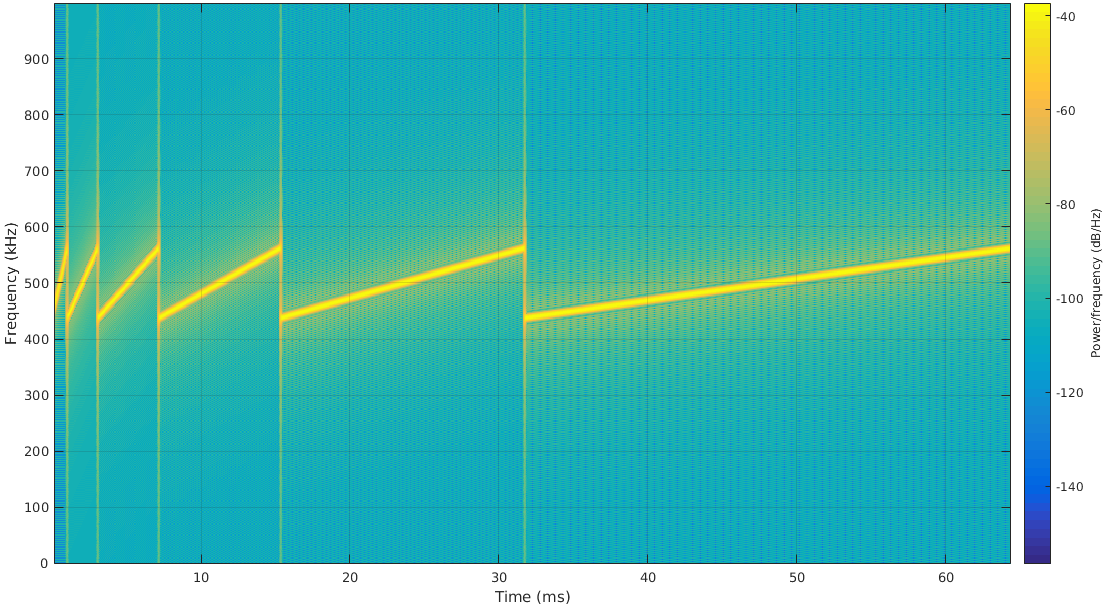
\includegraphics[width=.7\linewidth]{fig/lora_sf_comparasion.png}
\vspace*{4mm}
\caption{Spectrogram of different spreading factors (SF7 to SF12). \cite{sghoslya_lora}}
\label{fig:lora_sf_comparasion}
\end{figure}

When bandwidth and code rate are constant, as the spreading factor increases, the data rate decreases. Increasing the spreading factor makes the signal more resilient to noise thus increases the transmission range. Increasing the spreading factor also increases the transmission duration which increases the power consumption. Therefore, it is possible to trade between range and power consumption by changing spreading factor.

\begin{figure}
\centering
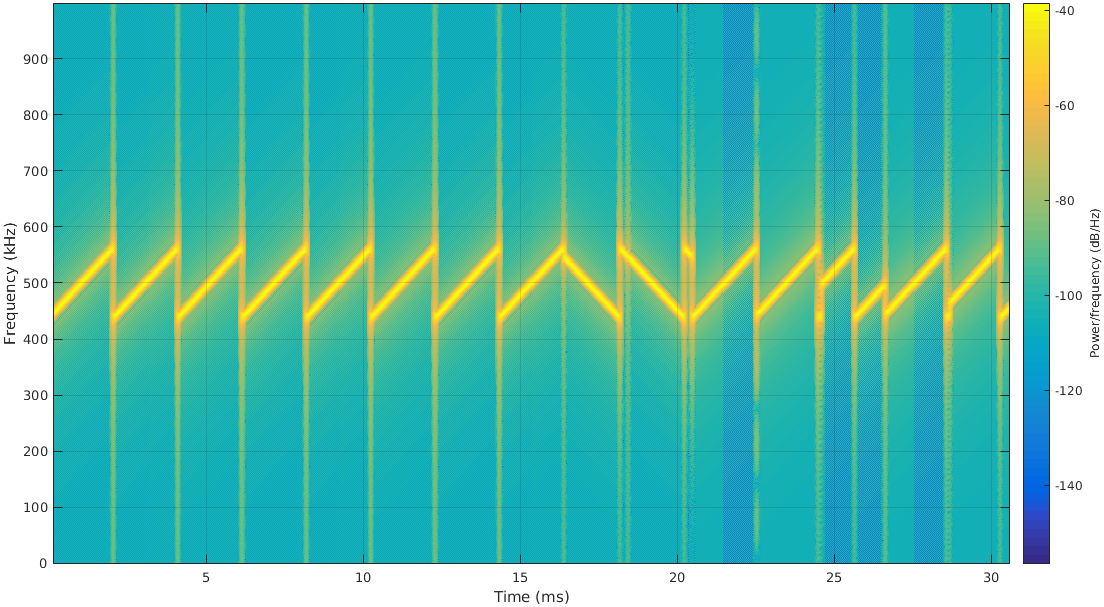
\includegraphics[width=.7\linewidth]{fig/lora_symbols.png}
\vspace*{4mm}
\caption{Spectrogram of a LoRa transmission. \cite{sghoslya_lora}}
\label{fig:lora_symbols}
\end{figure}

\subsection{Spreading Factor Assignment Issue}

Simultaneous different spreading factor transmissions are orthogonal to each other up to some extent. Which means that, a LoRa gateway can simultaneously receive multiple transmissions with different spreading factors. However, simultaneous transmissions with the same spreading factor may not be received by the gateway due to collision. For this reason, spreading factor assignment of nodes is crucial for network performance.

In a LoRaWAN network, initially, a node is not aware of how far away it is from a gateway. However, a node can guess the distance from a gateway by observing received signal power of a downlink transmission. If received signal power of a downlink transmission is too high, then node can decrease its next transmission spreading factor to decrease power consumption. This spreading factor assignment method is called lowest possible spreading factor assignment scheme for the rest of the thesis. Lowest possible spreading factor assignment scheme is commonly used in LoRaWAN deployments. Also, a gateway can request from a node to decrease its spreading factor or transmit power.

In Figure \ref{fig:collision}, a LoRaWAN network deployed with a single gateway is illustrated. Different color rings represent achievable range of different spreading factors from the gateway and different color circles represent selected spreading factor of the nodes. The end devices close to the gateway will fall into the lowest spreading factor (SF7) area section. The end devices close to the gateway will probably select the lowest spreading factor most of the time. This causes a lot of collisions between same spreading factor transmissions. Hence the number of collisions will increase as the number of end devices close to the gateway increases.

\begin{figure}
\centering
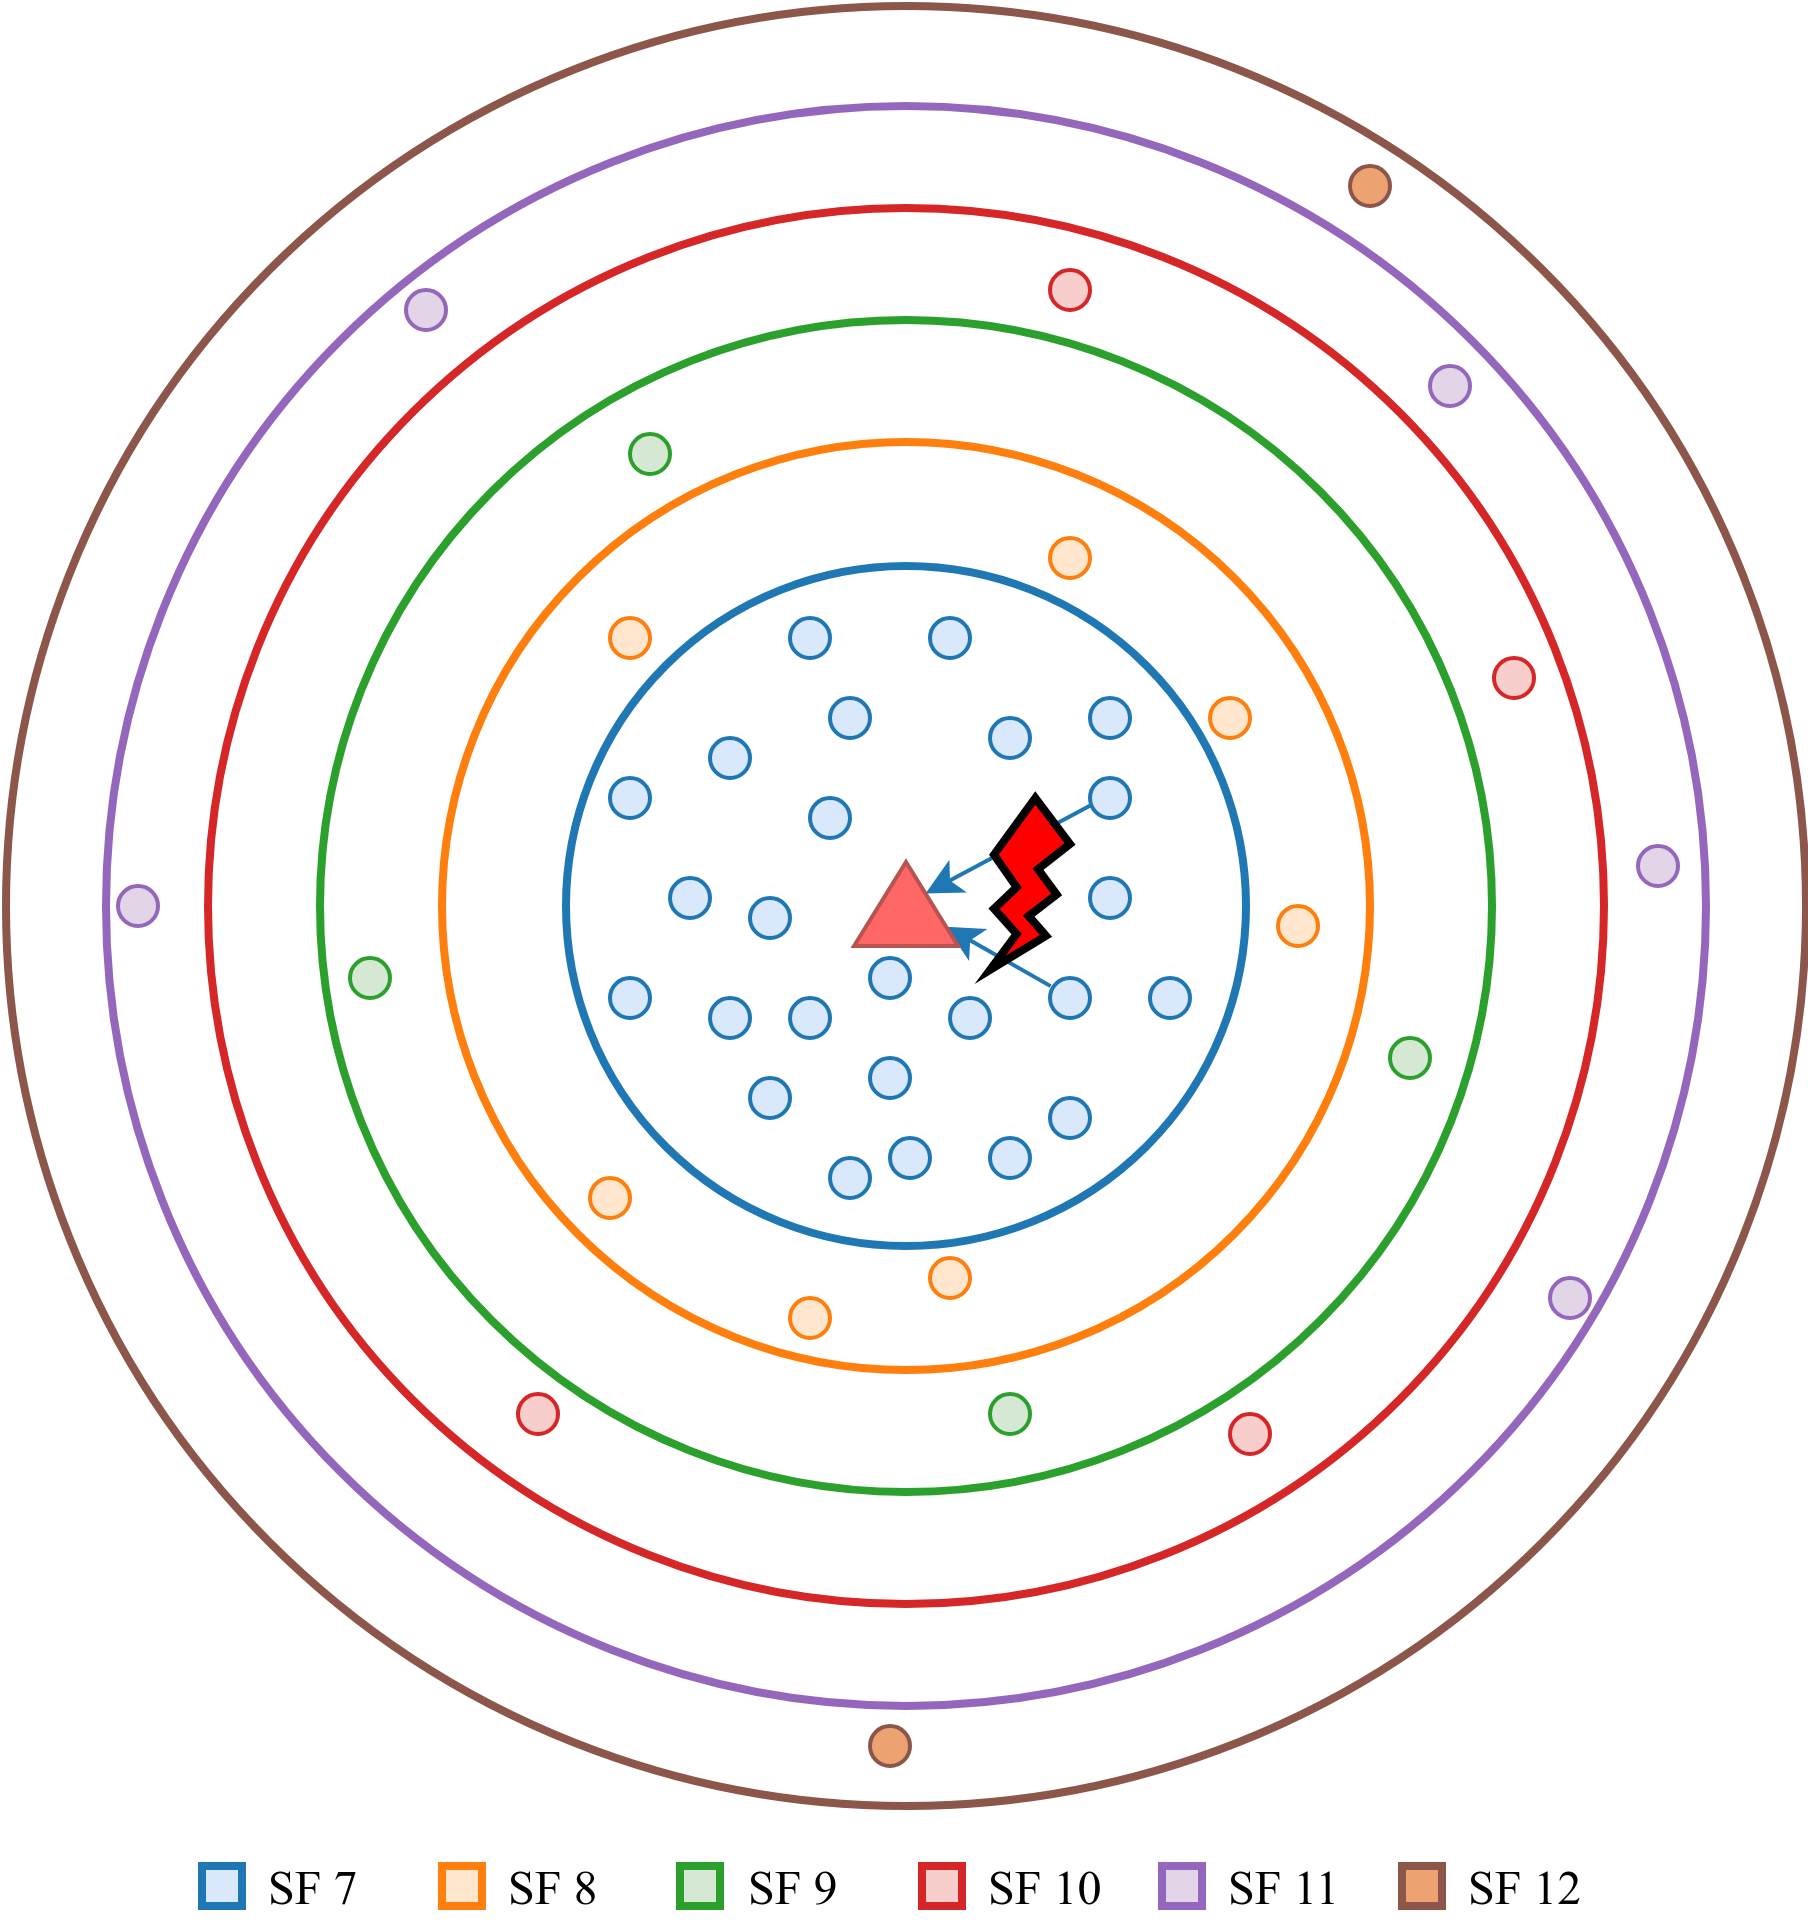
\includegraphics[width=.7\linewidth]{fig/lora_single_gw_collision.png}
\vspace*{5mm}
\caption{Collision between nodes close to the gateway.}
\label{fig:collision}
\end{figure}

\section{LoRaWAN}

LoRa has an open standard medium access control (MAC) layer protocol called LoRaWAN which is designed for large scale LoRa networks considering well known LPWAN challenges and their best practice solutions. LoRaWAN provides lightweight but powerful standard for wide range of LoRa IoT applications. LoRaWAN is developed and maintained by LoRa Alliance. LoRa Alliance is an open, non-profit organization dedicated to standardization of LoRaWAN. LoRaWAN provides inter-operability between different LoRa networks. LoRa can be used as a wireless link technology without complying LoRaWAN, however this would break inter-operability between different LoRa networks. LoRaWAN is based on pure ALOHA medium access which means that end nodes do not check whether the channel is free or not before transmission, accepting the possibility of a collision. A typical LoRaWAN network consists of three network entities which are end node, gateway and network server.

\subsection{End node}

LoRaWAN end node (EN) is a low power embedded device that only communicates to gateways. Single end node can communicate to multiple gateways. This communication architecture is called star of star network topology. LoRaWAN standard defines three classes for end devices which are Class A, Class B, and Class C. Different classes provide LPWAN solutions to different applications and deployments. Class A end nodes generate uplink transmission at any time and only receive a period of time after uplink transmission. Class B end nodes extend Class A behavior by adding scheduled receive windows for downlink transmission. Receive window is synchronized using a beacon packet transmitted by gateways. Class C end nodes extend Class A behavior by keeping receive window open all the time except uplink transmission. This provides Class C end nodes with low latency downlink communication, which requires more power consumption. In this thesis, only Class A end devices are considered since Class A behavior leads to the lowest power consumption.

\subsection{Gateway}

LoRaWAN gateway (GW) is a device that receive/transmit packets coming from/to end nodes. A typical gateway can receive from multiple channels at the same time. Gateways are usually connected to power grid, so power consumption of a gateway is insignificant in most of the deployments.

%TODO Adaptive Data Rate (ADR) TODO Page 8 of 101 \cite{lorawan.specification}.

\subsection{Network server}

LoRaWAN network server (NS) is a server that provides MAC layer processing. Network server routes messages from application to end nodes and vice versa. Network server can be used for tweaking end node parameters like channel, transmit power and spreading factor to increase network performance.

\begin{figure}
\centering
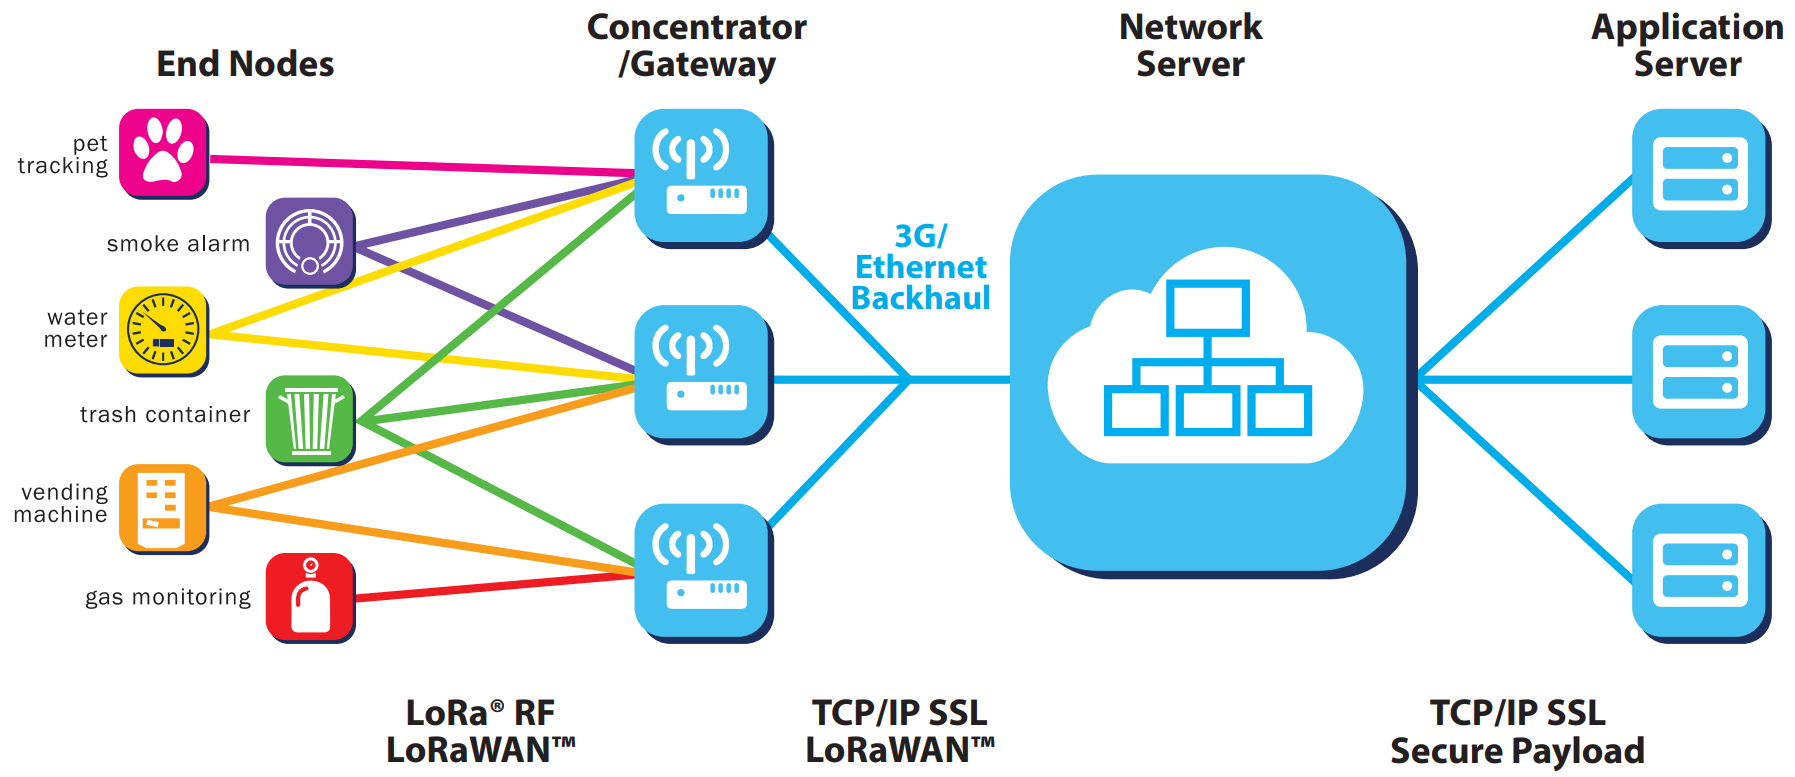
\includegraphics[width=\linewidth]{fig/lorawan_network.png}
\vspace*{4mm}
\caption{LoRaWAN network architecture. \cite{lorawan.technical.overview}}
\label{fig:lorawan_network}
\end{figure}
